\documentclass{beamer}

\mode<presentation>
{
	\usetheme{Warsaw}
	\usepackage{graphicx}
	% or ...	
	
	\setbeamercovered{transparent,invisible}
	\setbeamertemplate{navigation symbols}{}
	% or whatever (possibly just delete it)
}

\usepackage[english]{babel}
% or whatever
\usepackage{graphicx,subfigure}
\usepackage[utf8]{inputenc}
% or whatever

\usepackage{times}
\usepackage[T1]{fontenc}
% Or whatever. Note that the encoding and the font should match. If T1
% does not look nice, try deleting the line with the fontenc.
\usepackage{amsthm}
\newtheorem*{mylim*}{Limitations}
\usepackage{gensymb}
\usepackage{hyperref}
\hypersetup{
	colorlinks=true,
	linkcolor=blue,
	anchorcolor=blue,
	filecolor=blue,      
	citecolor=blue,
	urlcolor=blue
}
\usepackage{url,graphicx,subfigure}
\usepackage{listings}
\usepackage{color}
\usepackage{soul}
\usepackage{xspace}
\usepackage{pifont}
\usepackage{cite}
\usepackage{lipsum}% http://ctan.org/pkg/lipsum
\usepackage{algpseudocode}% http://ctan.org/pkg/algorithmicx
\usepackage{graphicx}
\usepackage[compatibility=false]{caption}% http://ctan.org/pkg/caption
\usepackage{booktabs}
\usepackage{url}
\usepackage{multirow}
\usepackage{pgfplots}
\usepackage{tikz}
\usetikzlibrary{matrix,fit,shapes,calc,positioning,shadows,arrows,shapes,backgrounds,decorations.markings,fadings}
\usepgfplotslibrary{statistics}
\usepackage[normalem]{ulem}
\useunder{\uline}{\ul}{}
\usepackage[skins]{tcolorbox}
\usepackage[linesnumbered,lined,boxed,ruled,vlined]{algorithm2e}
\usepackage[labelformat=empty]{caption}
\usepackage{color, colortbl}
\definecolor{Gray}{gray}{0.9}
\usepackage{amsmath,amssymb,amsfonts}

\hyphenation{op-tical net-works semi-conduc-tor}

\definecolor{comments}{rgb}{0.25,0.5,0.35}

\definecolor{brass}{rgb}{0.71, 0.65, 0.26}

\definecolor{SM}{rgb}{0.5,0,1}
\newcommand {\rsm} {\color{SM}}

\newcommand{\disp}{\insertframenumber/\inserttotalframenumber}

\newcommand{\backupbegin}{
	\newcounter{finalframe}
	\setcounter{finalframe}{\value{framenumber}}
}
\newcommand{\backupend}{
	\setcounter{framenumber}{\value{finalframe}}
}

\definecolor{antiquefuchsia}{rgb}{0.7, 0.1, 0.85}
\definecolor{airforceblue}{rgb}{0.36, 0.54, 0.66}
\definecolor{brass}{rgb}{0.71, 0.65, 0.26}
\definecolor{indiagreen}{rgb}{0.07, 0.53, 0.03}
\definecolor{darkorange}{rgb}{1.0, 0.55, 0.0}
\definecolor{navyblue}{rgb}{0.36, 0.54, 0.66}
\definecolor{darkred}{rgb}{0.55, 0.0, 0.0}

\newcommand{\REM}[1]{}
\newcommand{\todo}[1]{\textrm{\color{blue} #1}}
\newcommand{\sm}[1]{\textrm{\color{red} #1}}
\newcommand{\colosseum}{\textsf{Colosseum}\xspace}
\newcommand{\hansie}{\textsf{Hansie}\xspace}
\newcommand{\mahtab}{\textsf{Mahtab}\xspace}
\newcommand{\overallspeedup}{\todo{XXX}}

\resetcounteronoverlays{algocf}

\newcommand{\smr}[1]{\textrm{\color{black} #1}}
\newcommand{\sms}[1]{\textrm{\color{black} #1}}
\renewcommand{\ttdefault}{pcr}
\lstset{
	language=Java,
	escapechar=|,
	numbers=left,
	stepnumber=1,
	numbersep=5pt,
	numberstyle=\tiny\color{gray},
	backgroundcolor=\color{white},
	stringstyle=\fontsize{7.5}{7.5}\selectfont\ttfamily,
	keywordstyle=\ttfamily,
	showspaces=false,
	showstringspaces=false,
	showtabs=false,
	tabsize=2,
	captionpos=b,
	breaklines=true,
	breakatwhitespace=true,
	title=\lstname,
	basicstyle=\fontsize{7.5}{7.5}\selectfont\ttfamily,
	commentstyle=\color{red},
}
\newcommand{\ie}{i.e.}
\newcommand{\eg}{e.g.}
\newcommand{\aka}{a.k.a.}
\newcommand{\etal}{et al.}  % and colleagues
\newcommand{\CodeIn}[1]{{\small{\texttt{#1}}}}
\newcommand{\CodeInTab}[1]{{\scriptsize{\texttt{#1}}}}
\newcommand{\FancyIn}[1]{{\small{\textsc{#1}}}}
\newcommand{\MyComment}[1]{}
% common names
\newcommand{\reveng}{Reverse Engineering}

%% review original
\newcommand{\Fix}[1]{{\textbf{[[}\color{magenta}#1}\textbf{]]}}
\newcommand{\Mar}[1]{{\textbf{[[Marcelo:~}\color{red}#1}\textbf{]]}}
\newcommand{\SM}[1]{{\textbf{[[Shouvick:~}\color{blue}#1}\textbf{]]}}
\newcommand{\Den}[1]{[\textbf{Denini}:~{\color{brown} #1}]}

% \newcommand{\Fix}[1]{}
% \newcommand{\Mar}[1]{}
% \newcommand{\SM}[1]{}
% \newcommand{\Den}[1]{}

%% numbers
\newcommand{\configClasses}{\CodeIn{classes}}
\newcommand{\configMethods}{\CodeIn{methods}}
\newcommand{\configClassesAndMethods}{\CodeIn{classesMethods}}
\newcommand{\configClassesTab}{\CodeInTab{classes}}
\newcommand{\configMethodsTab}{\CodeInTab{methods}}
\newcommand{\configClassesAndMethodsTab}{\CodeInTab{classesMethods}}

\newcommand{\tname}{\textsc{PASTE}}

\def\denseitems{
   \itemsep1pt plus1pt minus1pt
   \parsep0pt plus0pt
   \parskip0pt\topsep0pt}

%% numbers and names
\newcommand{\OurURL}{\url{https://github.com/STAR-RG/paste}}
\newcommand{\NumProjects}{25}
\newcommand{\NumProjectsSpeedups}{13}
\newcommand{\FrequencySpeedups}{52} % NumProjectsSpeedups/NumProjects (13/25)
\newcommand{\SpeedupClassesAvg}{1.47}
\newcommand{\SpeedupClassesMedian}{1.59}
\newcommand{\SpeedupClassesMax}{2.28}
\newcommand{\SpeedupClassesMin}{0.93}
\newcommand{\NumRepeatsExperiment}{5}
\newcommand{\NumRepeatsManifest}{10}
\newcommand{\NumProjectsParExecFails}{11}
\newcommand{\NumProjectsParExecFailsPercentage}{44}
\newcommand{\NumStars}{200}
\newcommand{\NumTests}{300}
\newcommand{\NumFailsAtlasStageOneMethods}{147.2}
\newcommand{\NumFailsAtlasStageOneMethodsNoFraction}{141.2}
\newcommand{\NumFailsAtlasStageTwoMethods}{6}
\newcommand{\NumFailsClassesTotalStageOne}{402.6}
\newcommand{\NumFailsClassesAndMethodsTotalStageOne}{731.2}
\newcommand{\NumFailsMethodsTotalStageOne}{879.6}
\newcommand{\NumTestsClassificationSearchProcessorTest}{10}
\newcommand{\NumTestsMillionsPerDayGoogle}{150}
\newcommand{\EpochDuration}{45}
\newcommand{\NumDigitsSHA}{7}
\newcommand{\Processor}{Intel Core i5-1035G1 CPU @ 1.00GHz (base frequency)}
\newcommand{\NumCPUs}{8}
\newcommand{\NumCores}{4}
\newcommand{\RAMCapacity}{8}
\newcommand{\HardDiskCapacity}{512}
\newcommand{\KernelVersion}{5.4.0-42-generic}
\newcommand{\JavaVersion}{1.8.0\_282}
\newcommand{\BashVersion}{5.0.17}
\newcommand{\MavenVersion}{3.6.3}
\newcommand{\NumDepsChronicleQueue}{251}
\newcommand{\NumTestsChronicleQueue}{338}
\newcommand{\NumDepsCommonsCcollection}{2}
\newcommand{\NumTestsCommonsCcollection}{16,923}
\newcommand{\ForkscriptSurefirePatchedVersion}{\CodeIn{maven-surefire-plugin v3.0.0-M5}}
%% names


%% Configuration modes from ASE
\newcommand{\Seq}{\CodeIn{sequential}}
\newcommand{\SeqClassParMeth}{\configClasses}
\newcommand{\ParClassSeqMeth}{\configMethods}
\newcommand{\ParClassParMeth}{\configClassesAndMethods}
\newcommand{\Fork}{\Fix{?}}
\newcommand{\ForkSeq}{\Fix{?}}
\newcommand{\ForkParMeth}{\Fix{?}}
\newcommand{\pomf}{\CodeIn{pom.xml}}



\title[\color{white}ICSME 2021 Research Track Presentation.\hspace{14mm}\disp] % (optional, use only with long paper titles)
{Soundy Automated Parallelization\\of Test Execution}

\author[Shouvick Mondal \textit{et al}.] % (optional, use only with lots of authors)
{\underline{Shouvick Mondal}, Denini Silva, Marcelo d'Amorim\\\vspace{2mm}
{\scriptsize IIT Madras (India), UFPE (Brazil), UFPE (Brazil)}
\\\vspace{2mm}
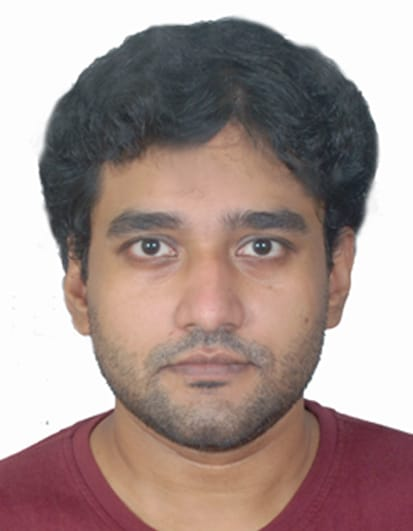
\includegraphics[width=0.13\textwidth]{images/shouvick2.jpg}~~~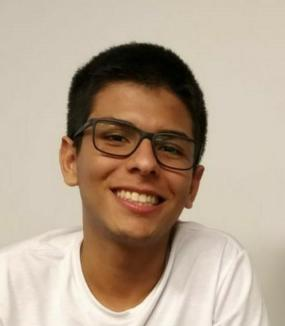
\includegraphics[width=0.15\textwidth]{images/denini.jpg}~~~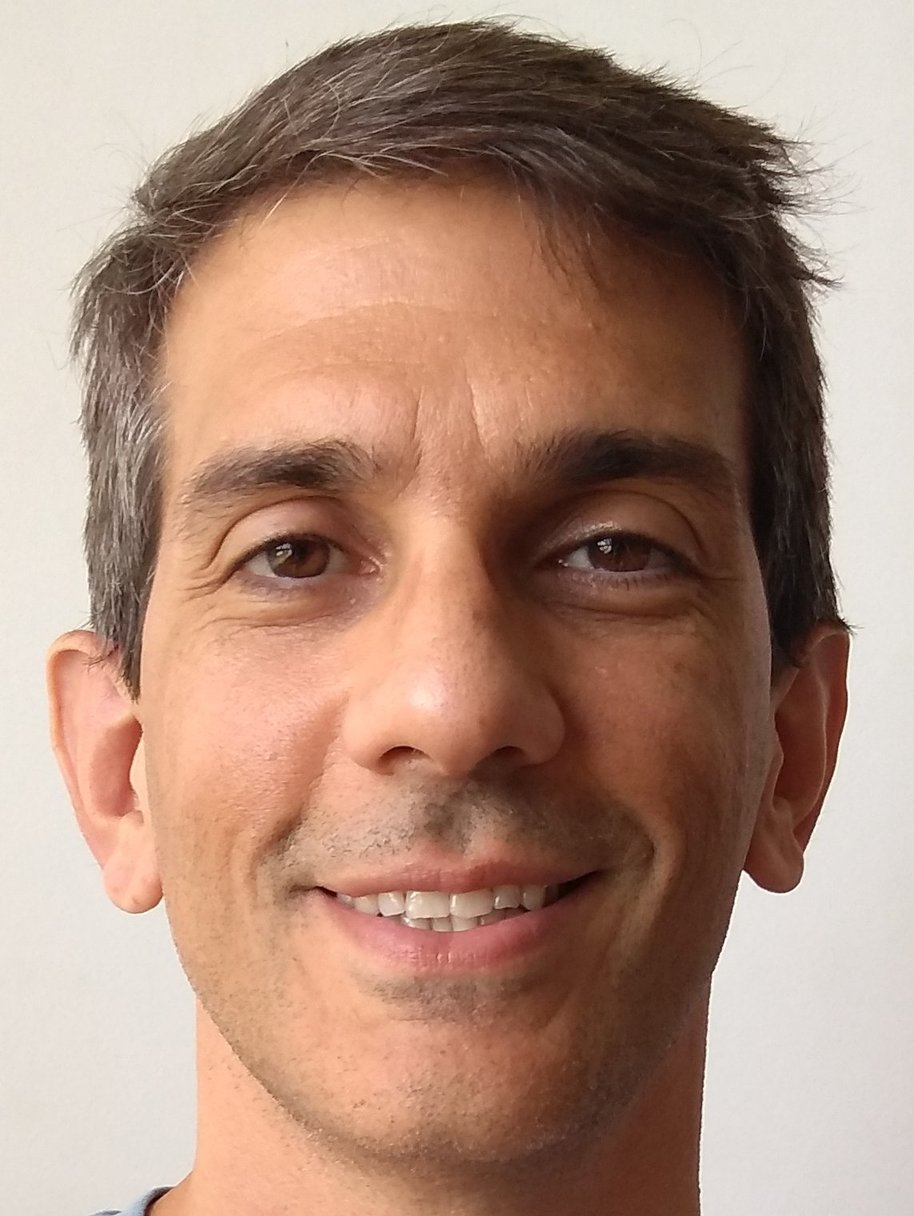
\includegraphics[width=0.13\textwidth]{images/marcelo.jpg}}
\date{ICSME 2021 (Virtual Event)\\{\scriptsize September 27 -- October 1}} % (optional, should be abbreviation of conference name)

%======================================================================================================

\begin{document}

\begingroup
\renewcommand{\disp}{}
\begin{frame}
	\titlepage
\end{frame}
\endgroup

\addtocounter{framenumber}{-1}

\begin{frame}{Context: software evolution and regression testing}
\vspace{-3.75mm}
\begin{center}
	{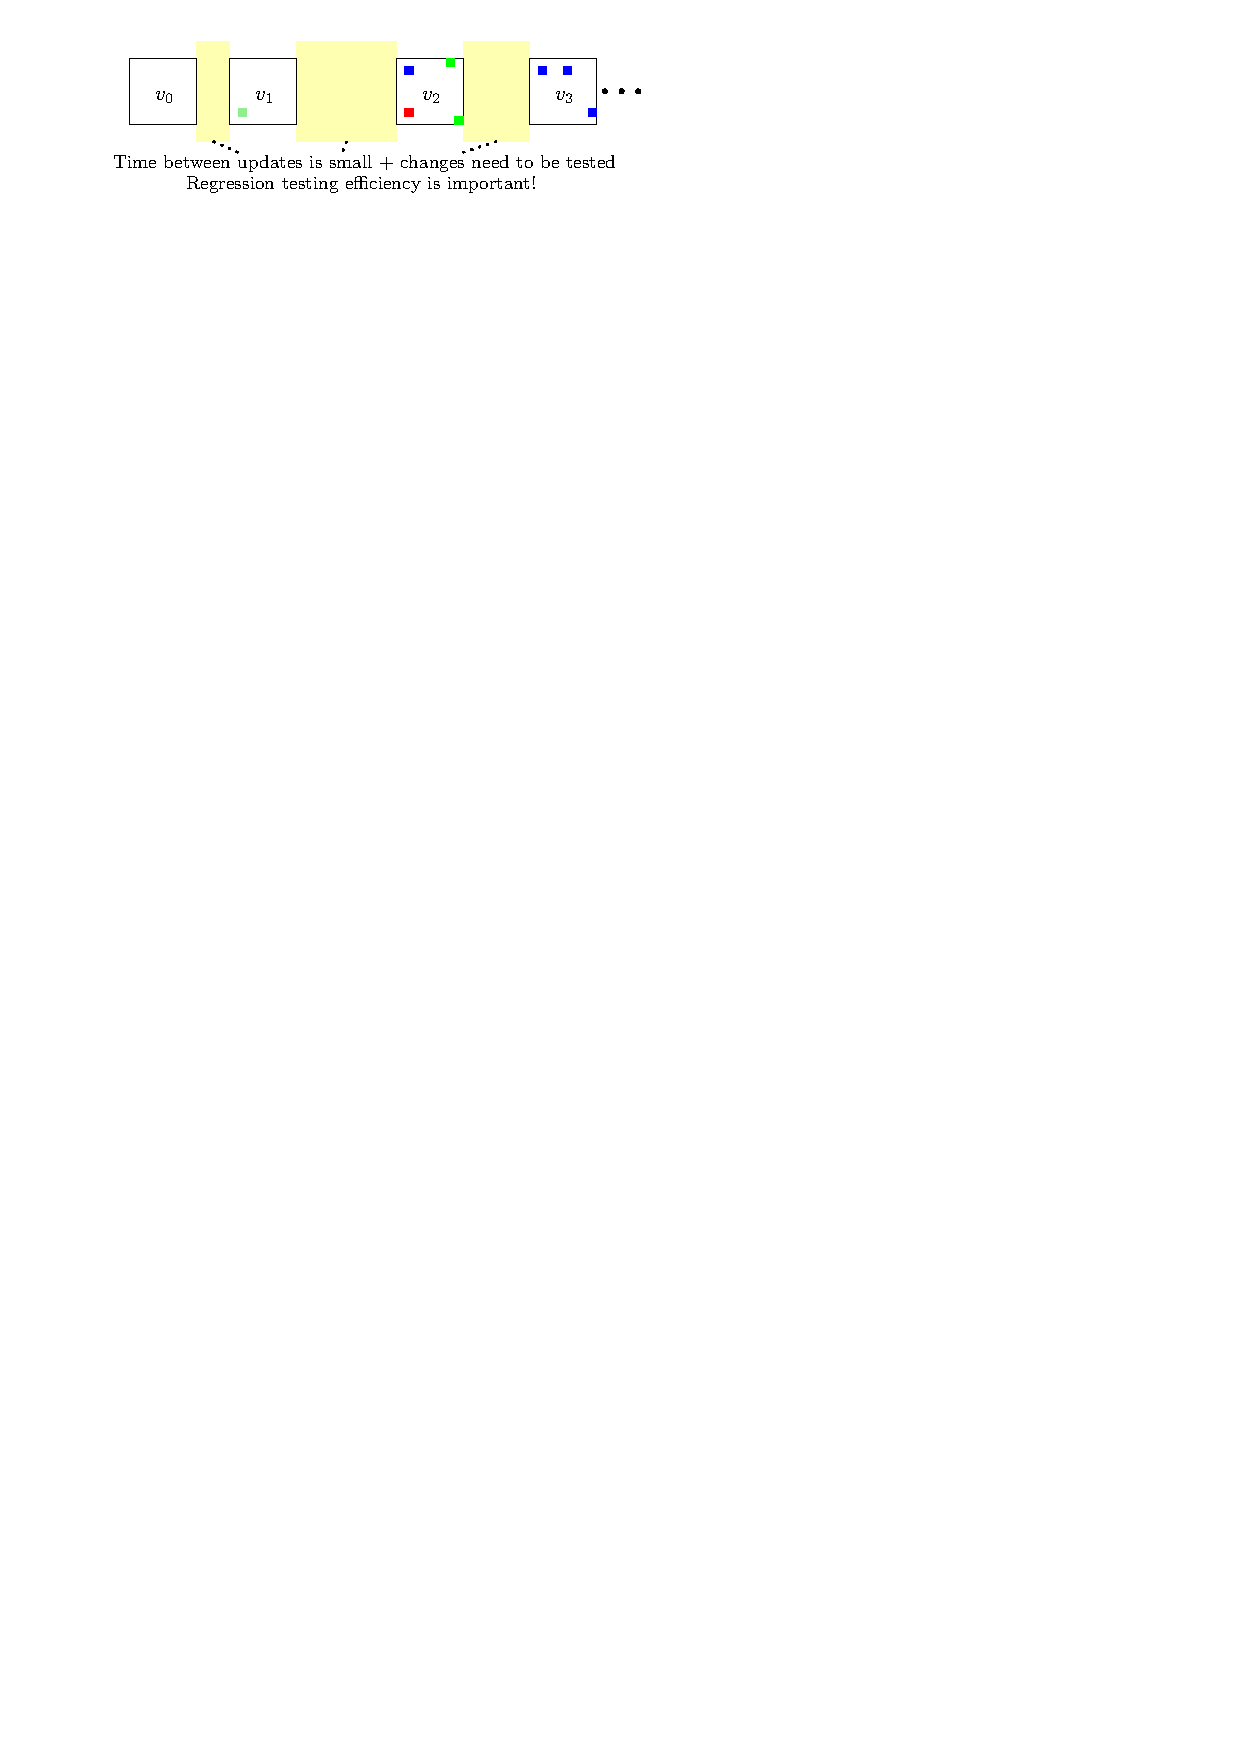
\includegraphics[width=\linewidth]{images/evolution.pdf}}
\end{center}
\vspace{-4mm}
\pause
{\textit{RetestAll}: execute all test-cases sequentially? ({\color{red}\textit{expensive}!})}\pause\\
Industrial example: RetestAll took seven weeks to complete!\onslide<3->\footnotemark\\\pause
\textit{Sophisticated solutions}
\begin{itemize}
	\item{{\small Regression test {\rsm selection} (RTS).}\onslide<4->\footnotemark}\pause
	\item{{\small Regression test {\rsm prioritization} (RTP).}\onslide<5->\footnotemark}\pause
	\item{{\small Test-suite {\rsm reduction} (TSR).}\onslide<6->\footnotemark}\pause
	\item{\textbf{\color{blue}\textit{Test-execution parallelization}} (\textit{is less explored}...).\onslide<7->\footnotemark}
\end{itemize}
\vfill
\only<3->{\footnotetext[1]{\fontsize{3.5}{3.5}\selectfont\textbf{Source}: S. Elbaum et al., \textit{Prioritizing Test Cases for Regression Testing}, ISSTA 2000.}}
\only<4->{\footnotetext[2]{\fontsize{3.5}{3.5}\selectfont\textbf{Source}: M. Gligoric et al., \textit{Ekstazi: Lightweight Test Selection}, ICSE 2015.}}
\only<5->{\footnotetext[3]{\fontsize{3.5}{3.5}\selectfont\textbf{Source}: S. Elbaum et al., \textit{Test Case Prioritization: A Family of Empirical Studies}, TSE 2002.}}
\only<6->{\footnotetext[4]{\fontsize{3.5}{3.5}\selectfont\textbf{Source}: G. Rothermel et al., \textit{Empirical Studies of Test-Suite Reduction.}, STVR 2002.}}
\only<7->{\footnotetext[5]{\fontsize{3.5}{3.5}\selectfont\textbf{Source}: J. Candido et al., \textit{Test suite parallelization in open-source projects: A study on its usage and impact.}, ASE 2017.}}
\end{frame}

\begin{frame}{Test parallelization levels}
\centering
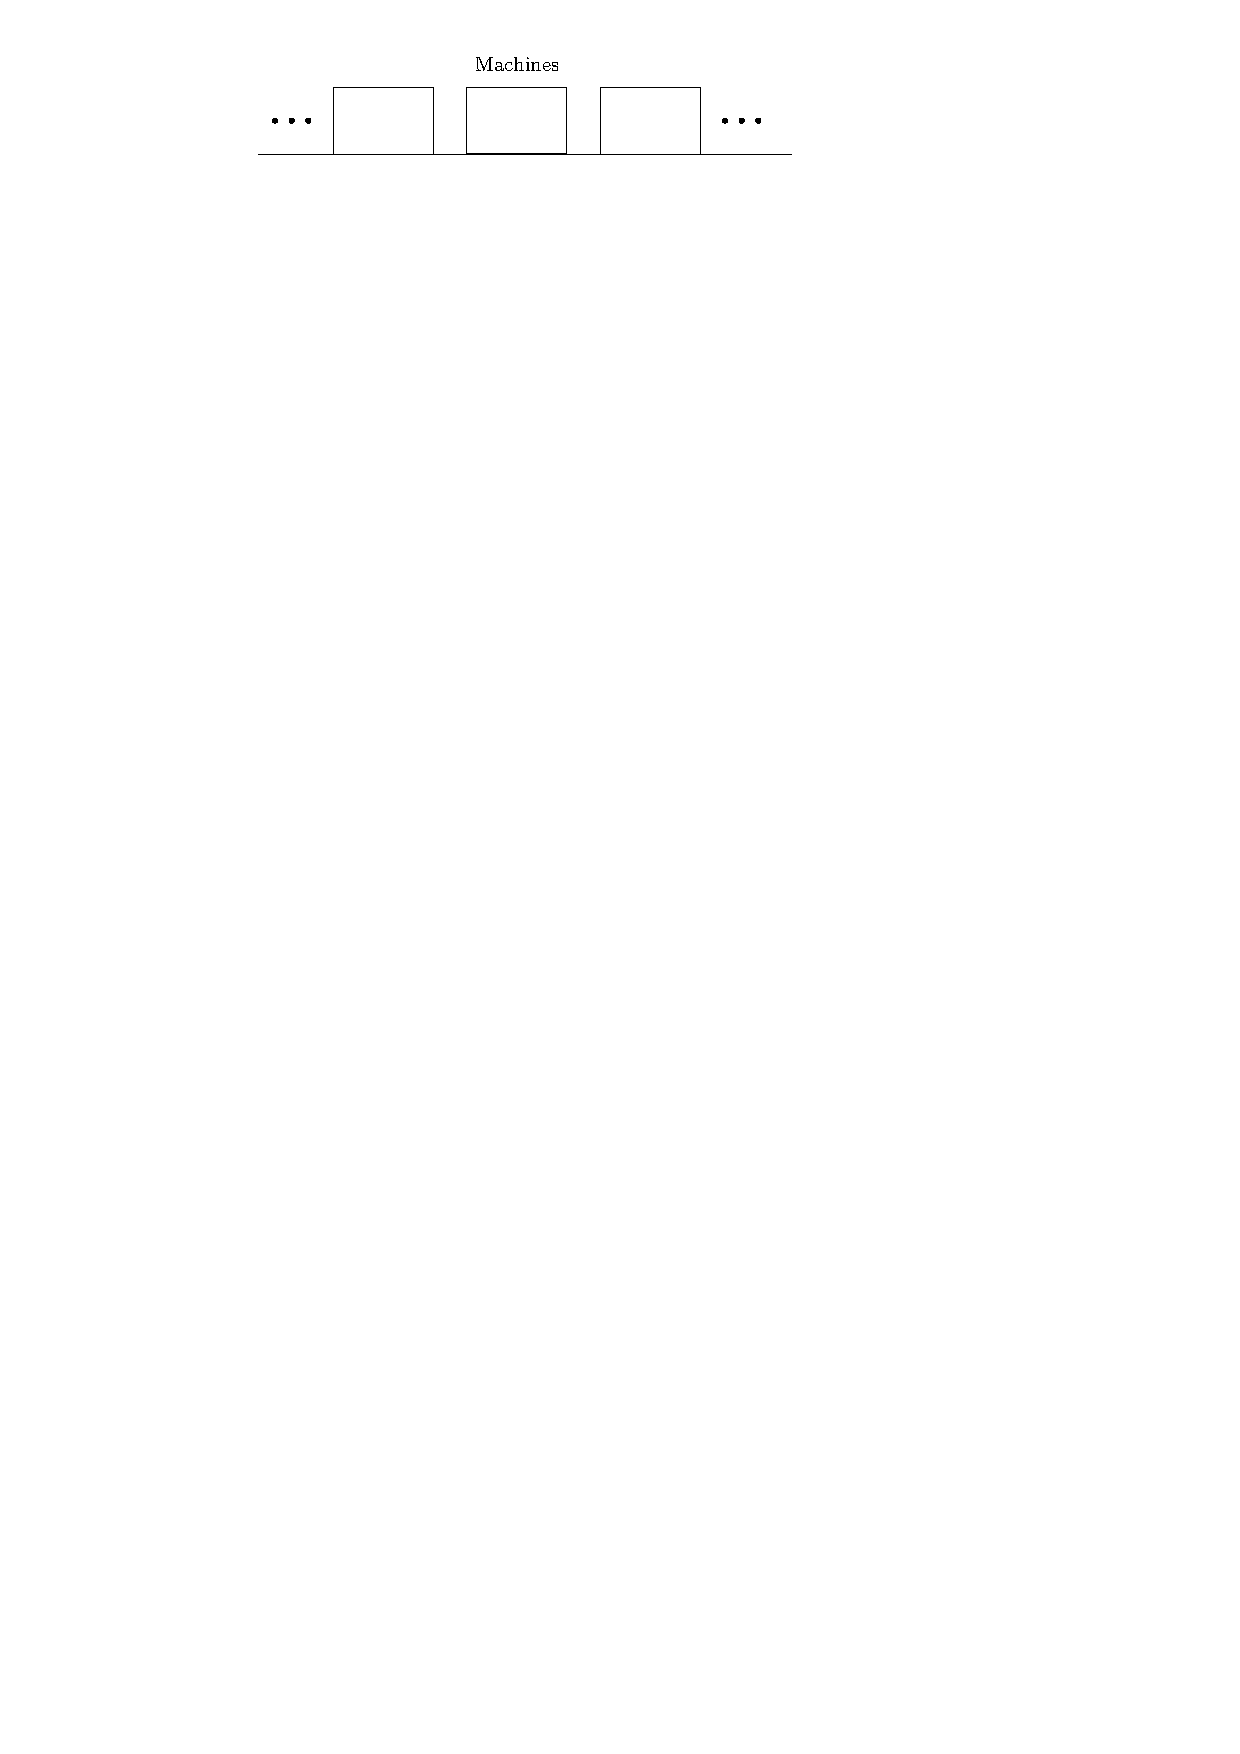
\includegraphics[width=\linewidth,page=1]{images/intro.pdf}
\vfill
{\color{white}In this work, we focus on \textit{CPU} and \textit{thread} level parallelism.}
\vfill
\vfill
{\fontsize{5}{5}\selectfont\textbf{Source}: J. Candido et al., \textit{Test suite parallelization in open-source projects: A study on its usage and impact}, ASE 2017.}
\end{frame}

\begin{frame}{Test parallelization levels}
\centering
\includegraphics[width=\linewidth,page=2]{images/intro.pdf}
\vfill
{\color{white}In this work, we focus on \textit{CPU} and \textit{thread} level parallelism.}
\vfill
\vfill
{\fontsize{5}{5}\selectfont\textbf{Source}: J. Candido et al., \textit{Test suite parallelization in open-source projects: A study on its usage and impact}, ASE 2017.}
\end{frame}

\begin{frame}{Test parallelization levels}
\centering
\includegraphics[width=\linewidth,page=3]{images/intro.pdf}
\vfill
{\color{black}In this work, we focus on \textit{CPU} and \textit{thread} level parallelism.}
\vfill
\vfill
{\fontsize{5}{5}\selectfont\textbf{Source}: J. Candido et al., \textit{Test suite parallelization in open-source projects: A study on its usage and impact}, ASE 2017.}
\end{frame}

\begin{frame}{Test flakiness: a major issue due to parallelization}
\begin{center}
{\{{\color{blue}\textbf{Test dependencies}, \textbf{Data-races}}\}$\rightarrow$\{{\color{red}\textbf{flakiness}}\}}
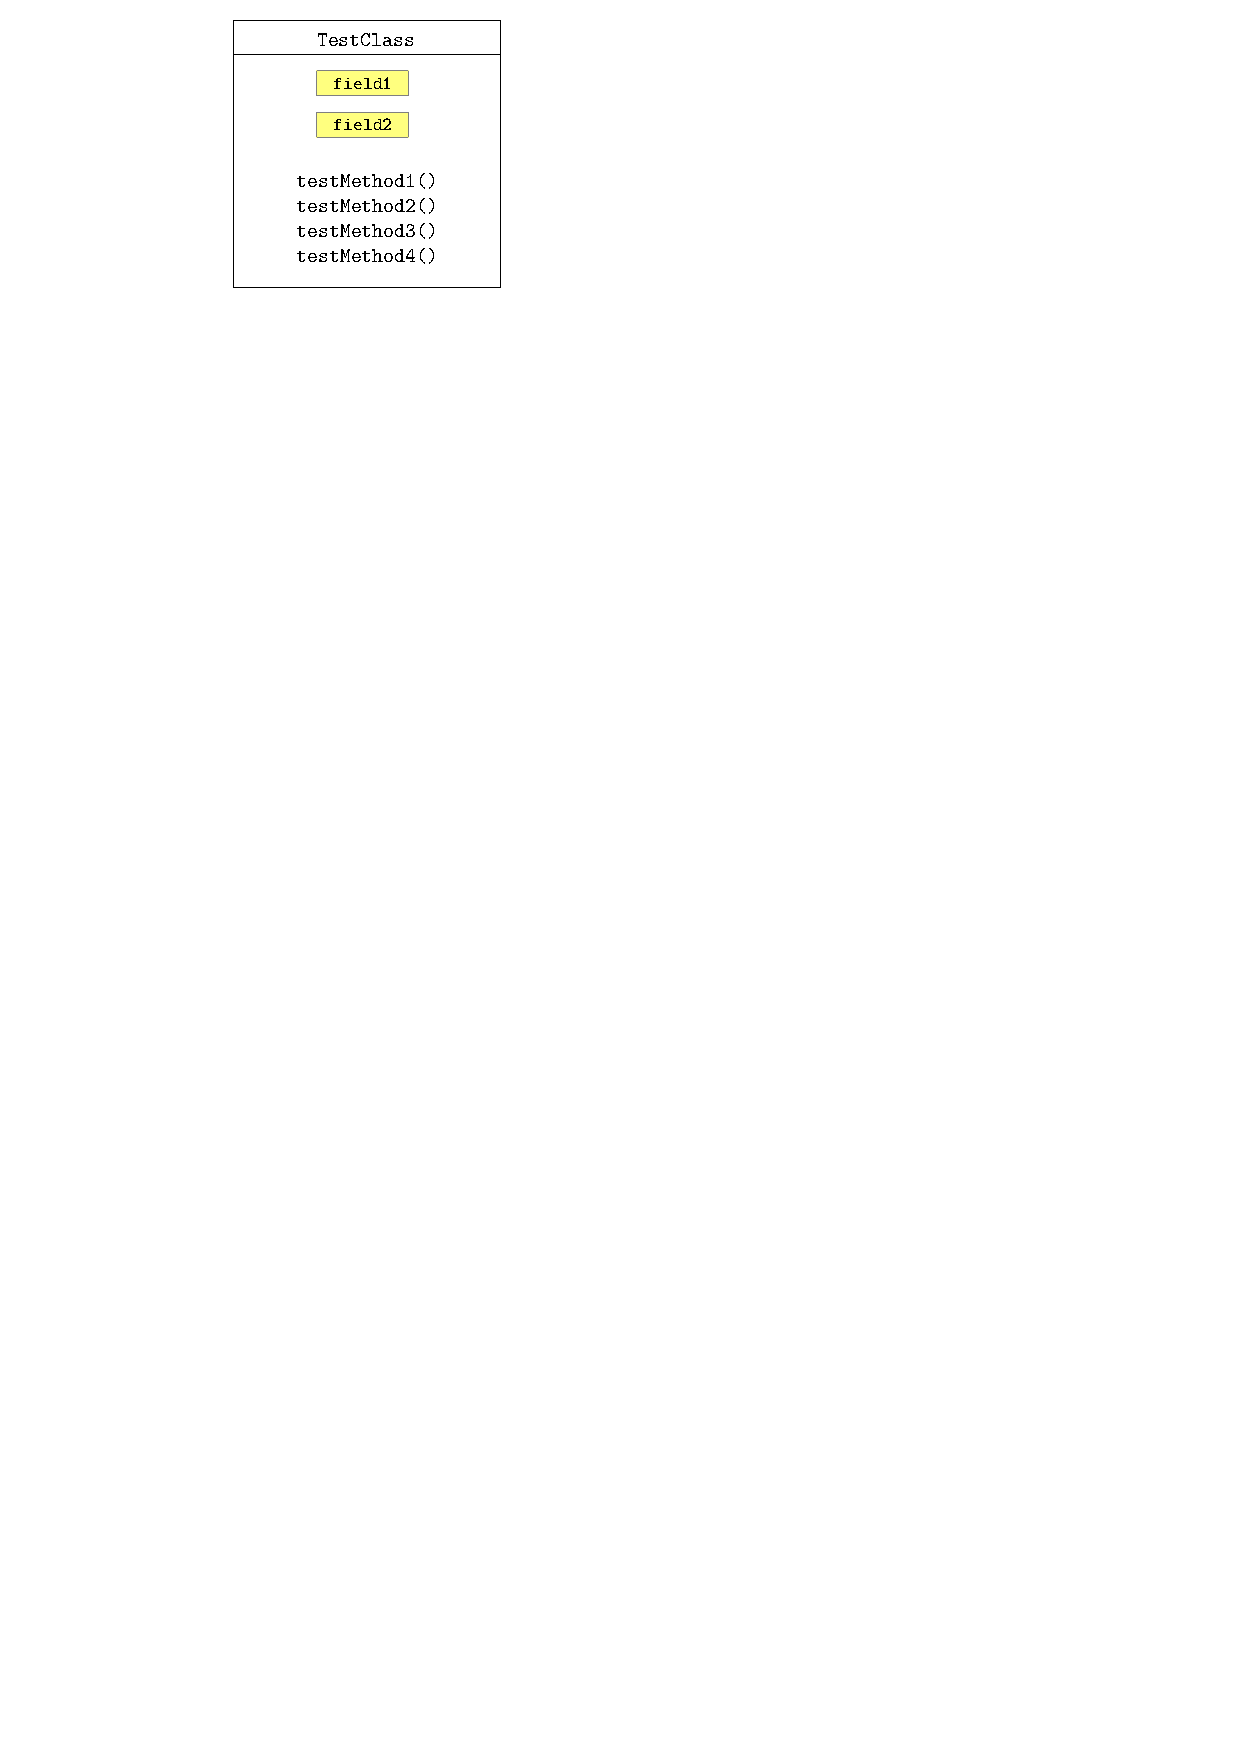
\includegraphics[width=0.6\linewidth,page=1]{images/flakes.pdf}
\end{center}
\end{frame}

\begin{frame}{Test flakiness: a major issue due to parallelization}
	\begin{center}
{\{{\color{blue}\textbf{Test dependencies}, \textbf{Data-races}}\}$\rightarrow$\{{\color{red}\textbf{flakiness}}\}}
		\includegraphics[width=0.6\linewidth,page=2]{images/flakes.pdf}
	\end{center}
\end{frame}

\begin{frame}{Test flakiness: a major issue due to parallelization}
	\begin{center}
{\{{\color{blue}\textbf{Test dependencies}, \textbf{Data-races}}\}$\rightarrow$\{{\color{red}\textbf{flakiness}}\}}
		\includegraphics[width=0.6\linewidth,page=3]{images/flakes.pdf}
	\end{center}
\end{frame}

\begin{frame}{Test flakiness: a major issue due to parallelization}
	\begin{center}
{\{{\color{blue}\textbf{Test dependencies}, \textbf{Data-races}}\}$\rightarrow$\{{\color{red}\textbf{flakiness}}\}}
		\includegraphics[width=0.8\linewidth,page=4]{images/flakes.pdf}
	\end{center}
\end{frame}

\begingroup
\renewcommand{\disp}{}
\begin{frame}
	\begin{center}
		{\rsm Test dependency detection}: \textit{can it aid test parallelization}? 
	\end{center}
\end{frame}
\endgroup
\addtocounter{framenumber}{-1}

\begin{frame}{Test dependency detection can be costly!}
	State-of-the-art dependency detector: PRADET (ICST 2018).
	\vfill
	\fbox{\rsm \textbf{PRADET}}
	\begin{itemize}
		\fontsize{11}{11}\selectfont
		\item[]{\underline{\textbf{Step 1} (costs $x$)}: {\rsm Sequential execution} to record original test ordering.}\pause
		\item[]{\underline{\textbf{Step 2} (costs $y$)}: {\rsm Dynamic data-flow analysis} collect data dependencies.}\pause
		\item[]{\underline{\textbf{Step 3} (costs $z$)}: {\rsm Iterative refinement} to keep problematic dependencies.}\pause
	\end{itemize}
	\begin{center}
		\begin{tcolorbox}
			The overhead of {\rsm PRADET} was {\color{red} \textbf{substantially higher than sequential execution itself}} ($y+z>{x}$).\\\textit{\textbf{NOT practical} to use PRADET} to aid test parallelization!
		\end{tcolorbox}
	\end{center}
\end{frame}

\begingroup
\renewcommand{\disp}{}
\begin{frame}
	\begin{center}
		Our approach: \textbf{\tname}\\
		{\textbf{\rsm PA}rallel-\textbf{\rsm S}equential \textbf{\rsm T}est \textbf{\rsm E}xecution}
	\end{center}
\end{frame}
\endgroup
\addtocounter{framenumber}{-1}

\begin{frame}{Our approach: \textbf{\tname}}
	
\textbf{\tname} builds on the observation:\\
{\rsm \textit{\textbf{broken test dependencies}}} that are manifested in parallel runs {\rsm \textit{\textbf{involve test cases from the same test class}}}.
	\begin{center}
		\begin{minipage}{0.48\linewidth}
			\centering
			\includegraphics[width=\linewidth,page=5]{images/flakes.pdf}
			%\vspace{1mm}
		\end{minipage}%
		\hfill
		\begin{minipage}{0.48\linewidth}
			\centering
			\includegraphics[width=\linewidth,page=6]{images/flakes.pdf}
			%\vspace{1mm}
		\end{minipage}\pause
	\begin{tcolorbox}
	\vfill
	\textbf{Handle flakiness} in test suites through:
	\begin{itemize}
		\item{\textbf{sequential} {\color{blue}\textbf{re-execution}} of \textbf{\color{indiagreen}test cases} \\({\textit{to avoid {\color{red}\textbf{data races}}}}).}
		\item{\textbf{sequential} {\color{blue}\textbf{re-execution}} of \textbf{\color{indiagreen}test classes} \\({\textit{to avoid {\color{red}\textbf{broken test dependencies}}}}).}
	\end{itemize}
	\end{tcolorbox}
	\end{center}
\end{frame}

\begin{frame}{\textbf{\tname{}}: the three-staged pipeline of test execution}
	\centering 
	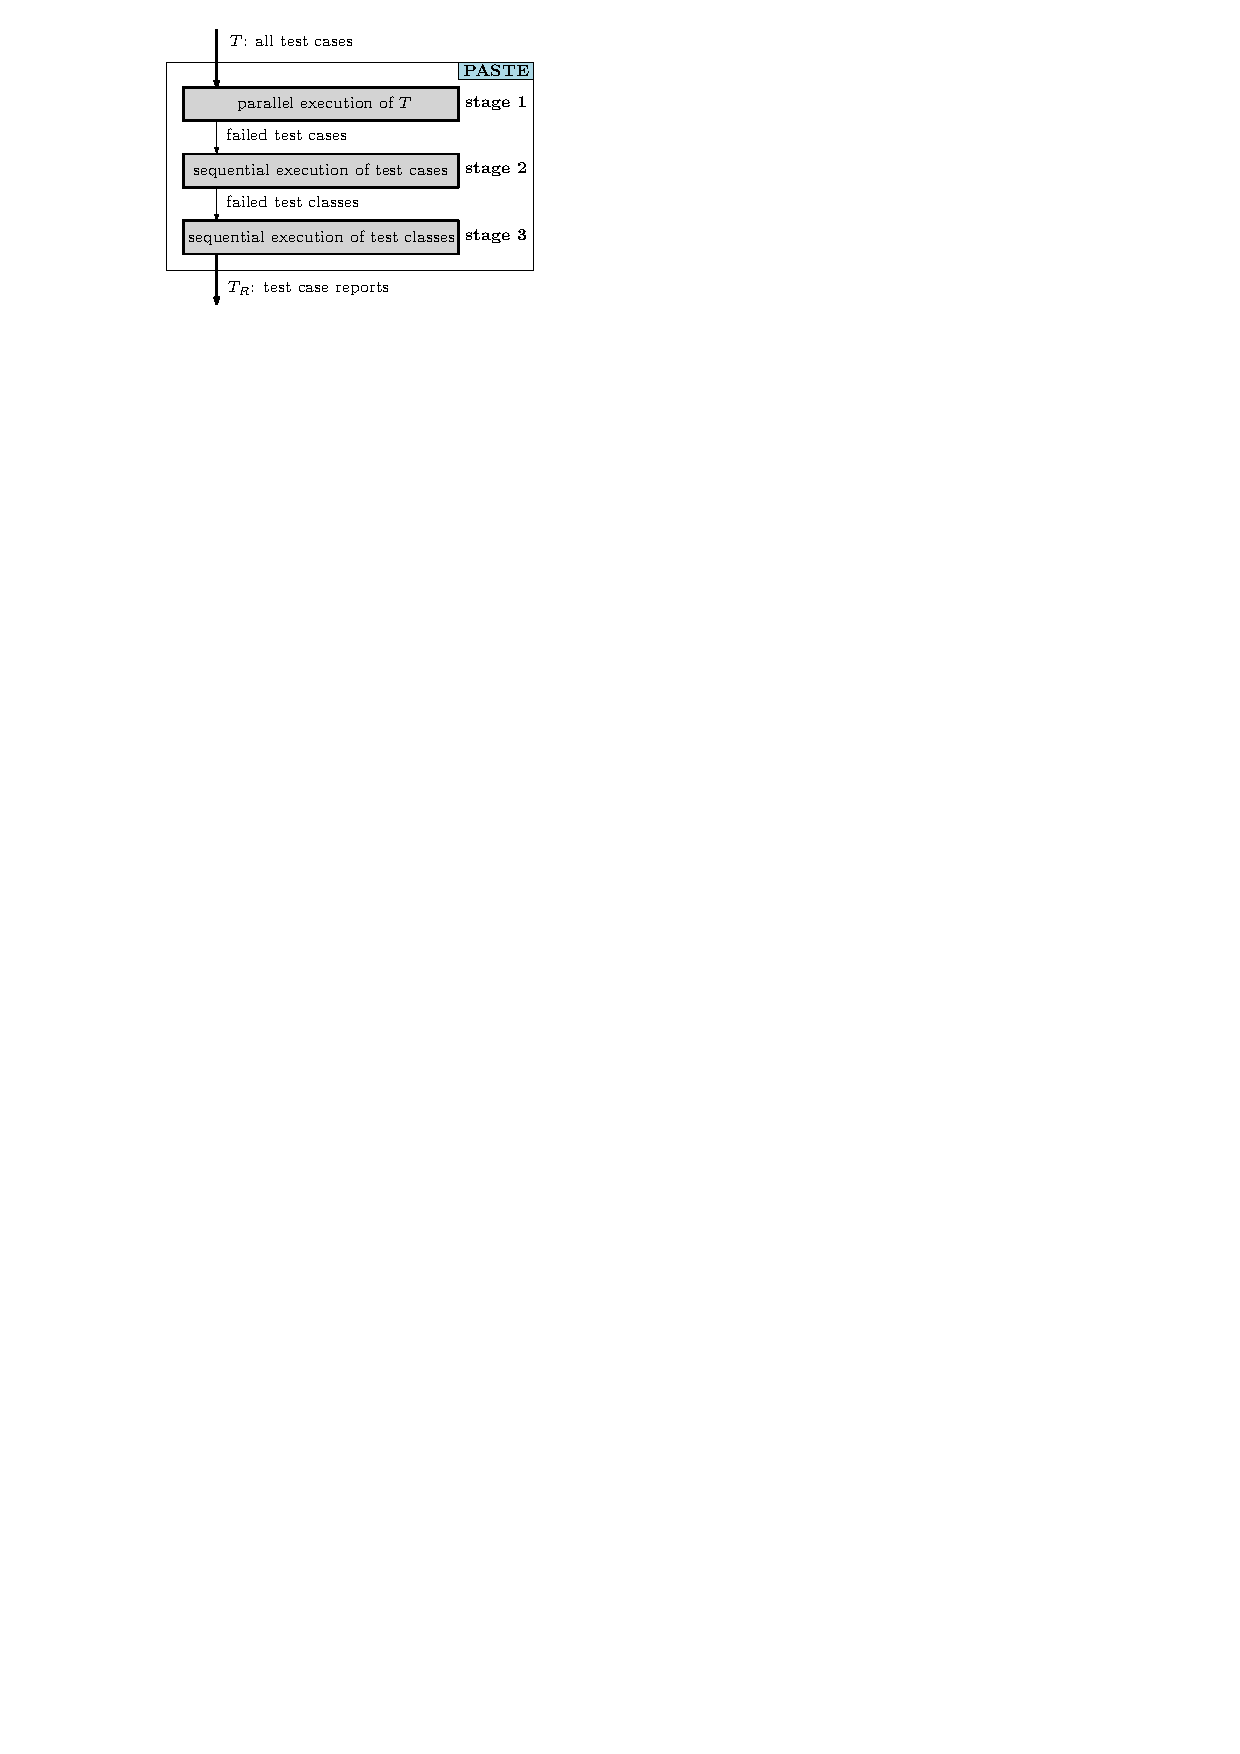
\includegraphics[width=0.8\linewidth,page=1]{images/soundy.pdf}
\end{frame}

\begin{frame}{Stage 1: parallel execution}
	\centering 
	\includegraphics[width=0.65\linewidth,page=2]{images/soundy.pdf}
\end{frame}

\begin{frame}{Stage 2: sequential re-execution of failed test cases}
	\centering 
	\includegraphics[width=0.65\linewidth,page=3]{images/soundy.pdf}
\end{frame}

\begin{frame}{Stage 3: sequential re-execution of failed test classes}
	\centering 
	\includegraphics[width=0.65\linewidth,page=4]{images/soundy.pdf}
\end{frame}

\begingroup
\renewcommand{\disp}{}
\begin{frame}
	\begin{center}
		{\rsm \textbf{The spectrum of soundness in parallelization}} 
	\end{center}
\end{frame}
\endgroup
\addtocounter{framenumber}{-1}

\begin{frame}{The spectrum of soundness in parallelization}
	
	{\textbf{\rsm Sound}: time invariant verdicts agree with sequential execution.}
	\begin{center}
		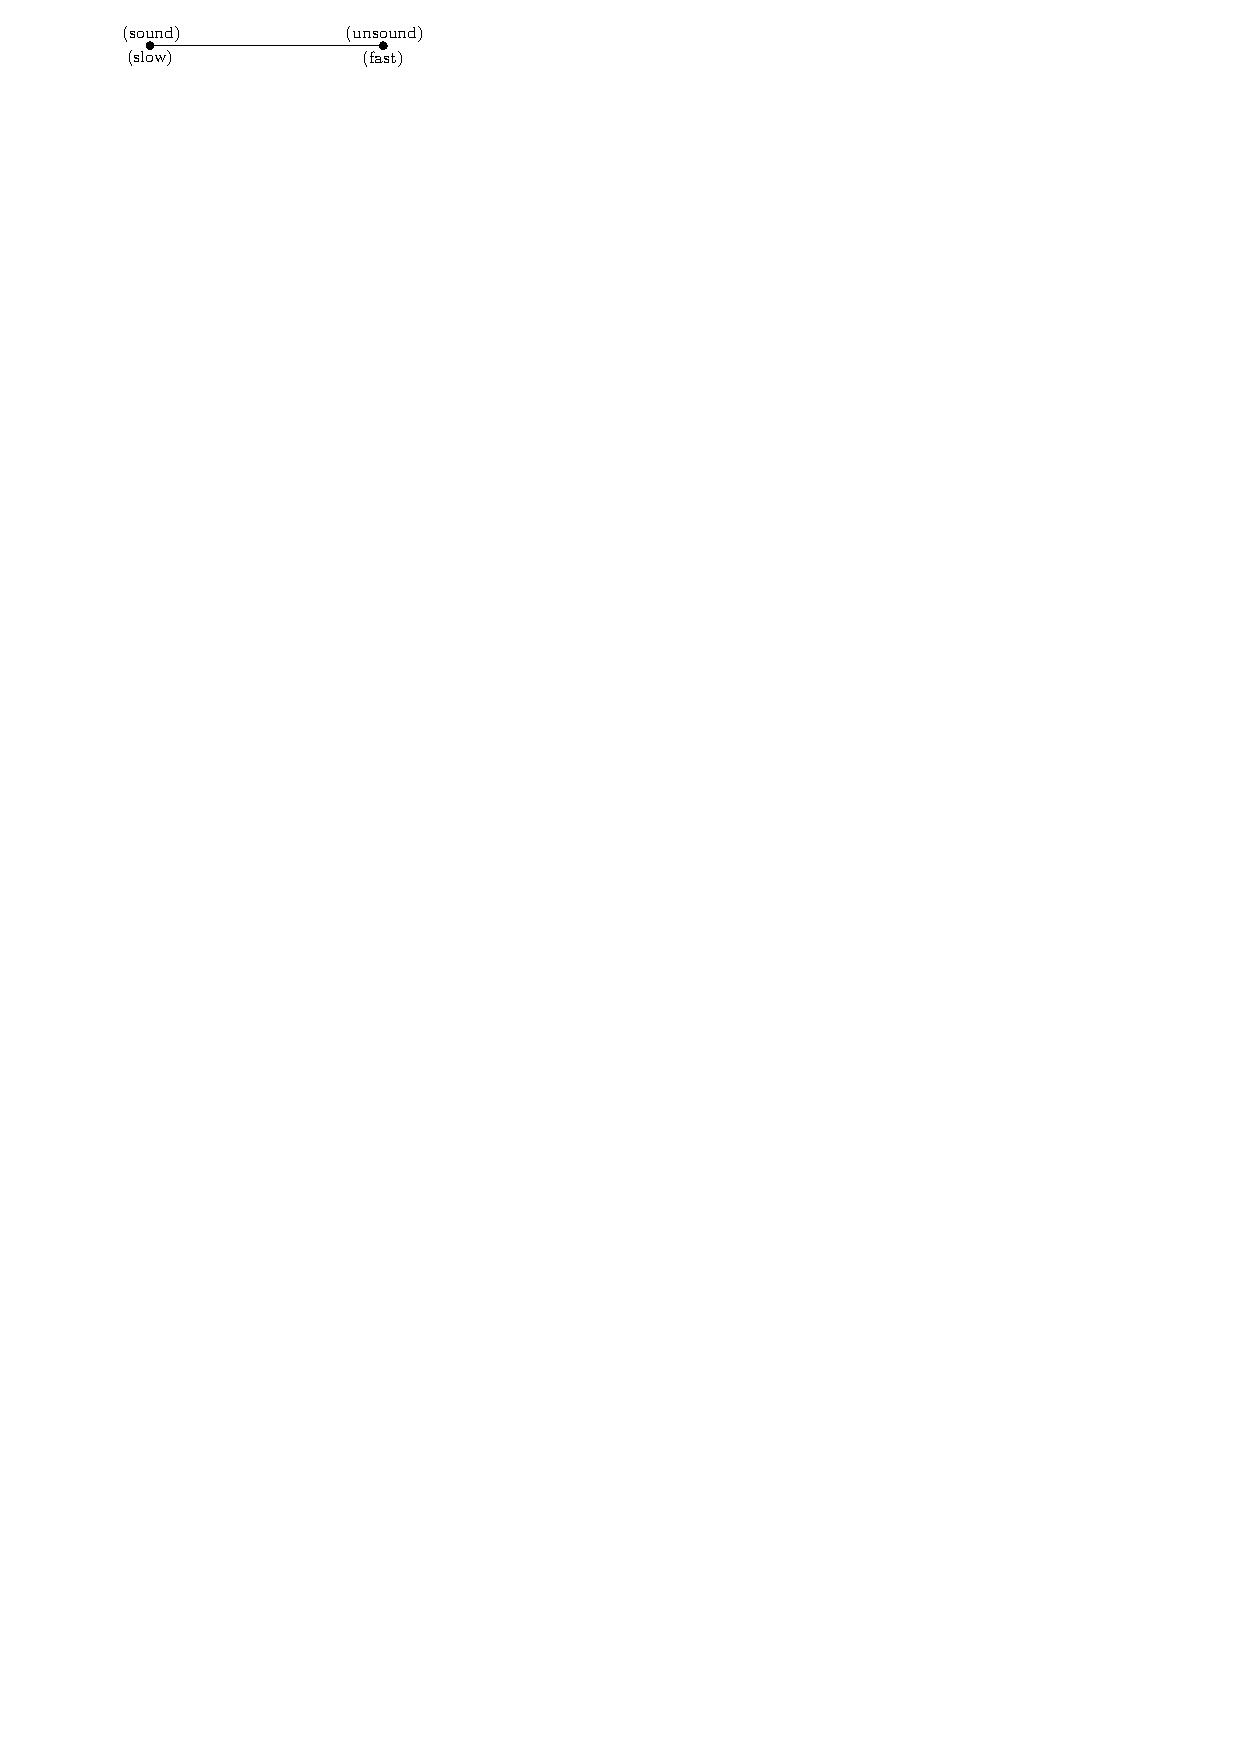
\includegraphics[width=0.8\linewidth,page=1]{images/spectrum.pdf}
		\vfill
		{\color{white}\tname{} does not provide the soundness guarantee but is reasonable enough to yield end-to-end acceleration!}
	\end{center}
\end{frame}

\begin{frame}{The spectrum of soundness in parallelization}
	
	{\textbf{\rsm Sound}: time invariant verdicts agree with sequential execution.}
	\begin{center}
		\includegraphics[width=0.8\linewidth,page=2]{images/spectrum.pdf}
		\vfill
		{\color{blue}\tname{} does not provide the soundness guarantee but is reasonable enough to yield end-to-end acceleration!}
	\end{center}
\end{frame}

\begingroup
\renewcommand{\disp}{}
\begin{frame}
	\begin{center}
		Experimental Setup
	\end{center}
\end{frame}
\endgroup
\addtocounter{framenumber}{-1}

\begin{frame}{Experimental Setup}
	\begin{itemize}
		\item{\textbf{\underline{Hardware}}: \textbf{\rsm \NumCPUs\ CPUs} (\textbf{\rsm \NumCores\ cores}, with \textbf{\rsm 2 threads per core}).}\pause
		\item{\textbf{\underline{Software}}: GNU \textbf{\rsm {Bash}} \BashVersion, and \textbf{\rsm {Maven}} \MavenVersion.}\pause
		\item{\textbf{\underline{Subjects}}: \textbf{\rsm \NumProjects\ Java projects} that use \textbf{\rsm {Maven}} and have at least \NumStars\ stars and \NumTests\ tests.}\pause
		\item{\textbf{\underline{No failures}}: Reran each test suite \NumRepeatsManifest\ times to \textbf{\rsm identify} and \textbf{\rsm eliminate tests failing} due to \textbf{\rsm non-determinism}.}\pause
		\item{\textbf{\underline{Parallel configuration}}: parameters in \textbf{\rsm Maven} and \textbf{\rsm JUnit}.}
	\end{itemize}
\end{frame}

\begingroup
\renewcommand{\disp}{}
\begin{frame}
	\begin{center}
		Research Questions
	\end{center}
\end{frame}
\endgroup
\addtocounter{framenumber}{-1}

\begin{frame}{RQ1 (feasibility \#1)}
	\textbf{\textit{Is it {\rsm feasible to use parallelization} options provided by the build system ``{\rsm out of the box}'' to run test suites?}}\pause
	\begin{center}
		\begin{tcolorbox}
			In \NumProjectsParExecFailsPercentage\% of the projects, no parallel configurations enabled a clean execution. Searching for the {\color{red}\textbf{parallel configuration for a clean execution is INFEASIBLE in general}}.
		\end{tcolorbox}
	\end{center}
\end{frame}

\begin{frame}{RQ2 (feasibility \#2)}
	\textbf{\textit{Is it {\rsm practical to use a test dependency analyzer} to partition test sets as to enable {\rsm sound} parallel execution?}}\pause
	\begin{center}
		\begin{tcolorbox}
			The runtime overhead of PRADET was substantially higher than that of the sequential execution itself. \textbf{\color{red} NOT PRACTICAL to use PRADET to aid test parallelization}.
		\end{tcolorbox}
	\end{center}
\end{frame}

\begin{frame}{RQ3 (effectiveness \#1)}
	\textbf{\textit{How {\rsm reliable} is \tname?}}
	\begin{center}\pause
		\begin{tcolorbox}
			Effective to circumvent the test flakiness provoked by test parallelization. There were \textbf{\color{red}no cases of provoked failure that ``survived'' the third stage} of \tname.
		\end{tcolorbox}
	\end{center}
\end{frame}

\begin{frame}{RQ4 (effectiveness \#2)}
	\textbf{\textit{What are the {\rsm speedups obtained} with \tname?}}
	\begin{center}\pause
		\begin{tcolorbox}
			We observed speedups in \FrequencySpeedups\% of the projects. The {\color{red}\textbf{configuration} \texttt{\textbf{classes}}} performed the best: {\color{red} \textbf{median}~\textbf{\SpeedupClassesMedian{}x}} (best: \SpeedupClassesMax{}x, average: \SpeedupClassesAvg{}x, worst: \SpeedupClassesMin{}x).
		\end{tcolorbox}
	\end{center}
\end{frame}

\begin{frame}{RQ4 (effectiveness \#2)}
	\vspace{-1.2cm}
	\begin{figure}
		\centering
		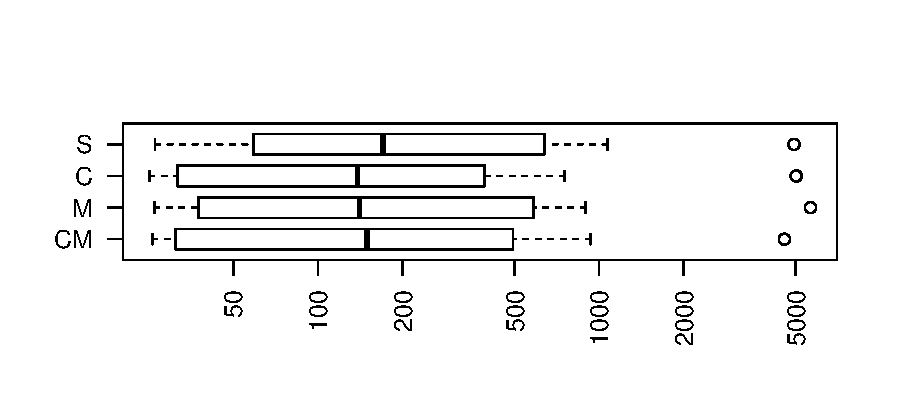
\includegraphics[width=\linewidth]{images/time.pdf}
		\vspace{-1.4cm}
		\caption*{Distribution of {\rsm \textbf{\tname{} running times (seconds)}} for Sequential (S) and each configuration (Classes (C), Methods (M), ClassesMethods (CM)).}
	\end{figure}
	\vspace{-1.25cm}\pause
	\begin{figure}
		\centering
		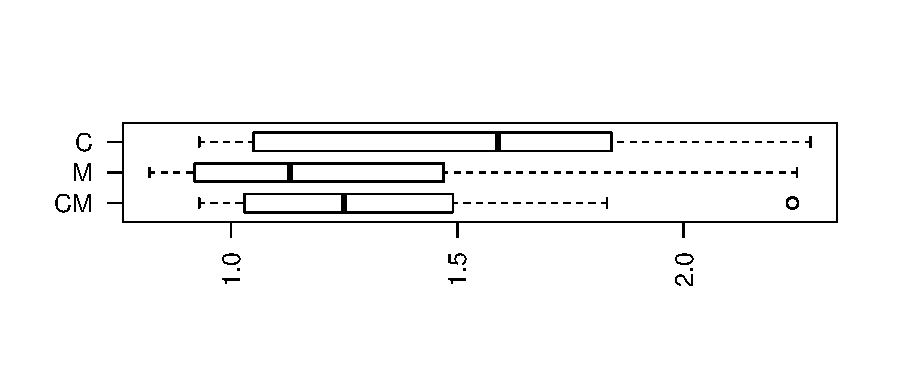
\includegraphics[width=\linewidth]{images/speedup.pdf}
		\vspace{-1.6cm}
		\caption*{Distribution of {\rsm \textbf{speedups}} for each configuration (Classes (C), Methods (M), ClassesMethods (CM)).}
	\end{figure}
\end{frame}

\begingroup
\renewcommand{\disp}{}
\begin{frame}
	\begin{center}
		Related Work
	\end{center}
\end{frame}
\endgroup
\addtocounter{framenumber}{-1}

\begin{frame}{Some recent approaches towards test parallelization}
	\begin{center}
		\fontsize{7.5}{7.5}
		{	
			\selectfont
			\setlength{\tabcolsep}{0.9mm}
			\centering
			\begin{tabular}{l|l|r|l}
				\hline
				{\textbf{Work--venue}} & {\textbf{Languages used}} & {\textbf{Speedup}} & {\textbf{Machine type}}\\
				\hline
				{} & {} & {} & {}\\
				{{\rsm ElectricTest}--FSE 2015} & {\rsm Java} & {Avg. $16.00\times$} & {Amazon EC2}\\
				{} & {} & {} & {}\\
				\hline
				{} & {} & {} & {}\\
				%{{\rsm GPU execution}--ASE 2014} & {CUDA and {\rsm C (subset)}} & {Max. $27.00\times$} & {GPU}\\
				{{\rsm ParTeCL} (GPU)--ISSTA 2017} & {OpenCL and {\rsm C (subset)}} & {Avg. $16.00\times$} & {GPU}\\
				{} & {} & {} & {}\\
				\hline
				{} & {} & {} & {}\\
				{Candido et al.--ASE 2017} & {\rsm Java} & {Avg. $3.53\times$} & {8 cores @ 3.60 GHz}\\
				%{} & {Avg. $1.90\times$} & {80 cores @ 2.20 GHz}\\
				{({\rsm multi-core})} & {} & {Avg. $4.20\times$} & {80 cores @ 2.20 GHz}\\
				{} & {} & {} & {}\\
				\hline
				{} & {} & {} & {}\\
				{\mahtab--JSS 2019} & {C++, LLVM, and {\rsm C}} & {Avg. $5.17\times$} & {40 cores @ 2.40 GHz}\\
				%{} & {Avg. $1.90\times$} & {80 cores @ 2.20 GHz}\\
				{({\rsm multi-core})} & {} & {G.M. $4.72\times$} & {40 cores @ 2.40 GHz}\\
				{} & {} & {} & {}\\
				\hline
			\end{tabular}
		}	
	\end{center}
	\centering
	%{\fontsize{9}{9}\selectfont We \underline{\textit{may get}} a {\color{indiagreen}\textbf{good speedup}}.}
\end{frame}

\begin{frame}{Conclusions}
	\begin{itemize}
		\item[]{\footnotesize We discussed {\rsm \textbf{\tname{}}}, a lightweight approach to {\rsm \underline{parallelize execution}} of test suites through the {\rsm \underline{sequential re-execution} of \textit{test cases}} (\textit{to avoid data races}) and the {\rsm \underline{sequential re-execution} of \textit{test classes}} (\textit{to avoid broken test dependencies}).}
	\end{itemize}
	\begin{center}
		\begin{figure}[!htb]
			\centering
			\begin{minipage}{0.475\textwidth}
				\centering
				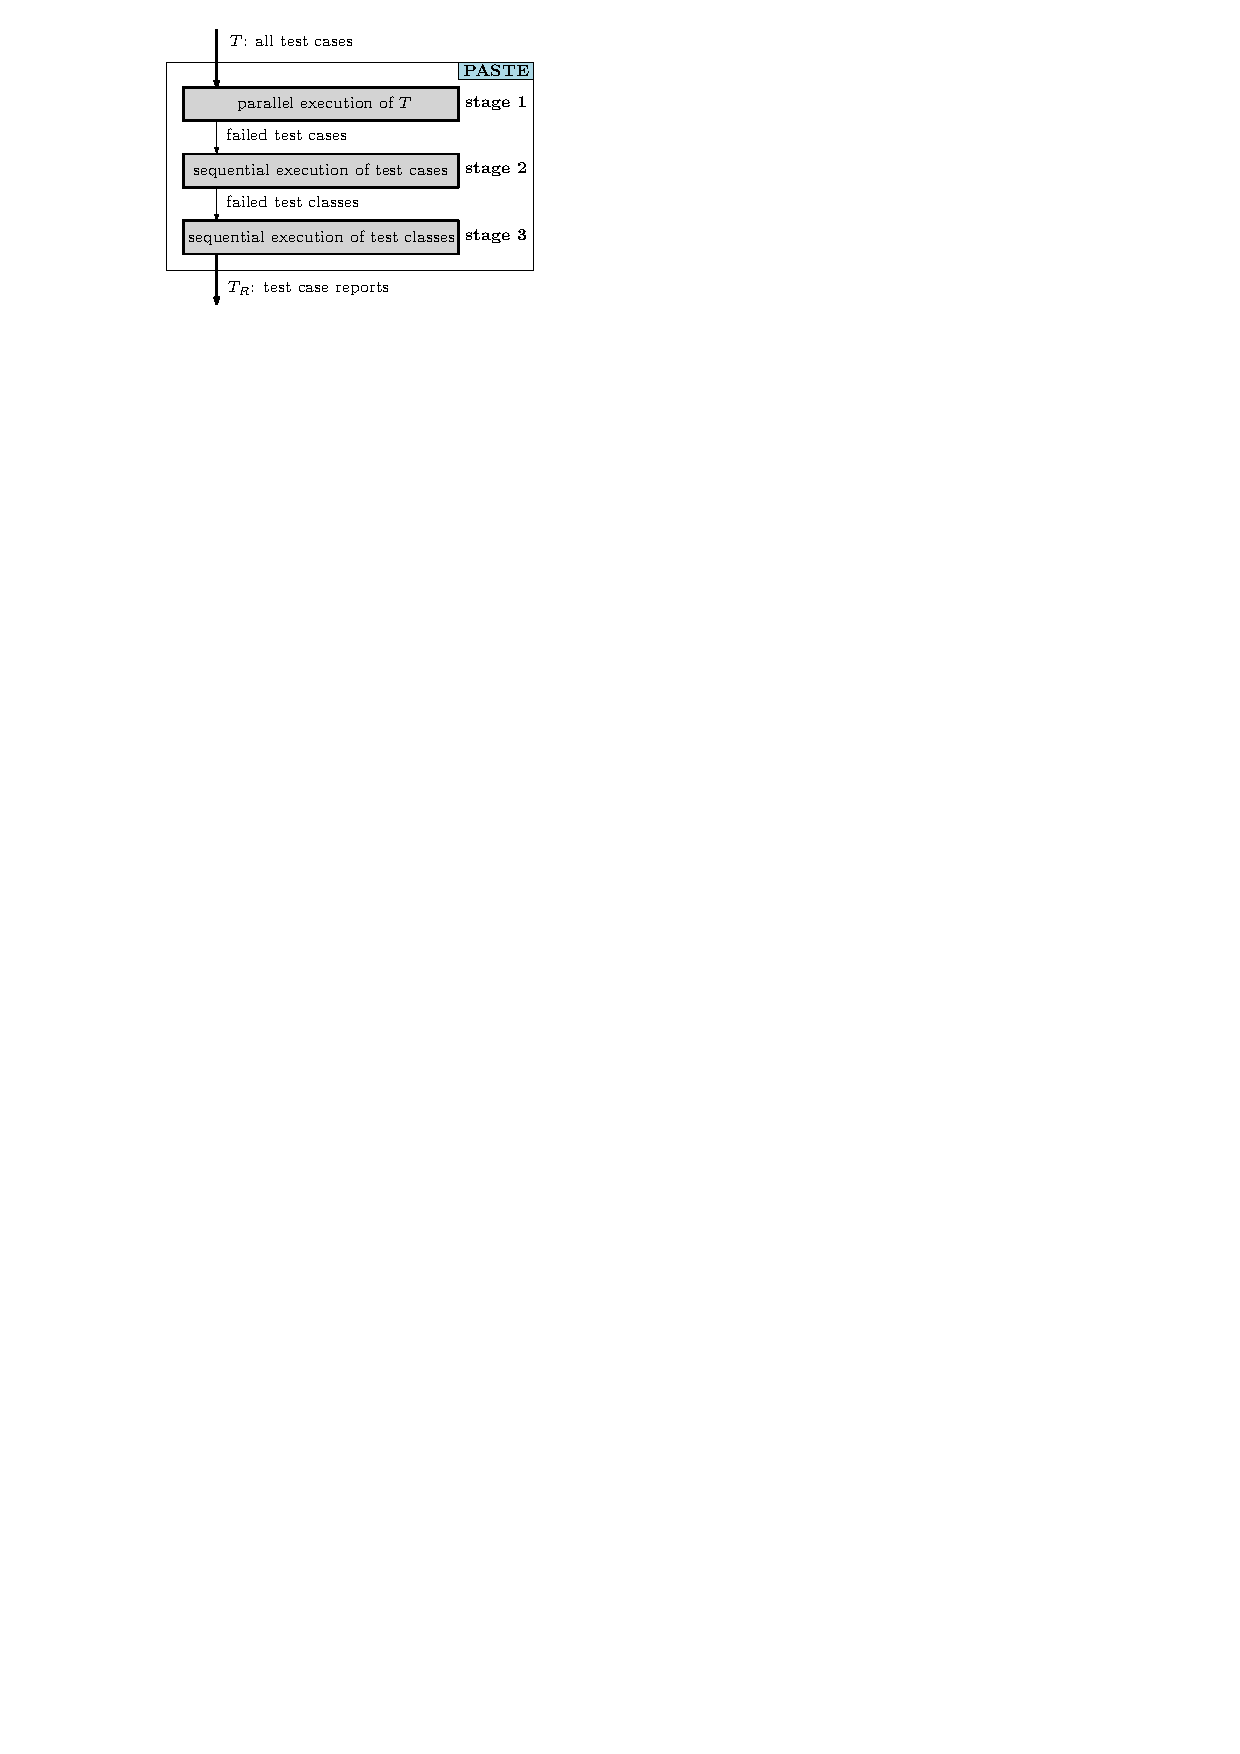
\includegraphics[width=\linewidth]{images/soundy.pdf}	
			\end{minipage}%
			\pause
			\begin{minipage}{0.5\textwidth}
				\centering
				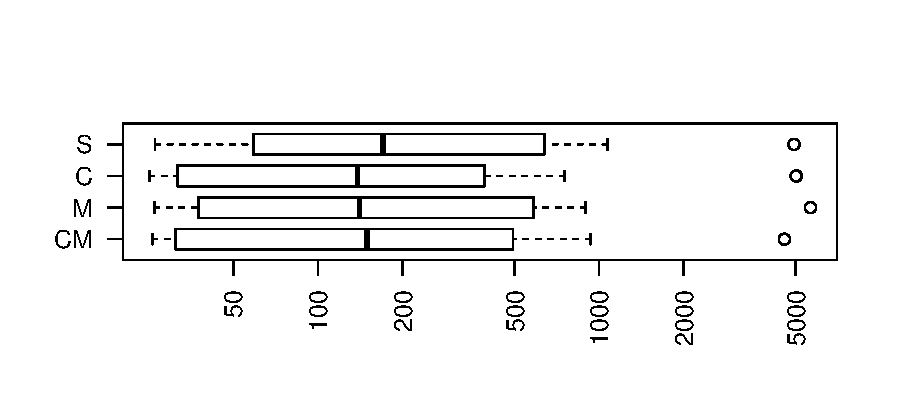
\includegraphics[width=1.175\linewidth]{images/time.pdf}\vspace{-1cm}
				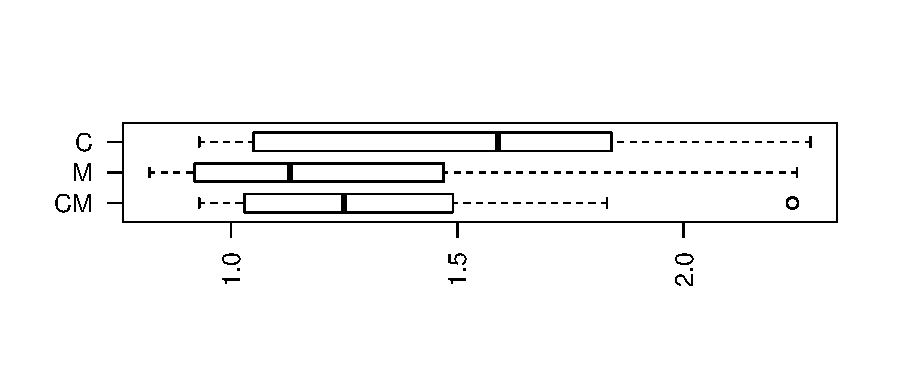
\includegraphics[width=1.175\linewidth]{images/speedup.pdf}	
			\end{minipage}
		\end{figure}
		\includegraphics[width=0.5\linewidth,page=2]{images/spectrum.pdf}
		\pause
		\hfill
		\begin{Large}
			Thank You
		\end{Large}
		\vfill
		\begin{footnotesize}
			Artifacts: \url{https://github.com/STAR-RG/paste}
		\end{footnotesize}
	\end{center}
\end{frame}

%======================================================================================================

\REM{

\renewcommand{\disp}{}

\appendix
\backupbegin

\begin{frame}
	\begin{center}
		{\huge Backup Slides}
	\end{center}
\end{frame}

\begin{frame}{TODOs for the slides...}
	\begin{itemize}
		\item[]{\textbf{Time split (in minutes)}:\\3 (context) + 3 (\tname{}) + 4 (eval, related, conclusion).}
		\vfill
		\item{\textbf{Be on point} about regression testing, avoid detail.}
		\item{\textbf{Mention briefly} about efficiency of reg. testing. RTS, RTP, TSR, parallelization (\textit{we focus here}): complementary + industry relevant + less explored academically.}
		\item{\textbf{Parallelization} (focus on two issues only):\\\{data-races, broken test dependencies\}$\rightarrow$\{flakiness\}.}
		\item{\textbf{Simplify example}: too convoluted currently! \textit{Simplify}..}
		\item{\textbf{Spectrum} (show explicitly: \textit{beautify}):\\(fast, unsound) ------ (\tname{}, soundy) ----- (slow, sound).}
		\item{\textbf{Simplify text}: keep only keywords + messages, no singleton bullet, max 2 lines per bullet.}
		\item{\textbf{Simplify RQs} (\textit{gray boxes only}): be on point, \textit{Simplify}..}
	\end{itemize}
\end{frame}

\begin{frame}{Context: software evolution and regression testing}
	
	{\rsm Consider manipulating a function}:\\
	$\{f(x)=2+x\}$ $\rightarrow$ $\{f'(x)=2*x\}$.\\
	\vspace{0.3cm}
	\pause
	Inputs (test-cases): {\rsm 2}, {\rsm 4}\\
	\textit{Expected} outputs: {\color{indiagreen}4}, {\color{indiagreen}6}\\\pause
	\textit{Observed} outputs: {\color{indiagreen}4}, {\color{red}8}\\
	\vspace{0.3cm}\pause
	{\color{indiagreen}Functionality}: $f({\rsm 2})=f'({\rsm 2})=\color{indiagreen}4$ is still intact.\\
	\vspace{0.3cm}\pause
	\vspace{-4mm}
	{\color{red} Failure} (functional discrepancy) revealed: $f({\rsm 4})\neq f'({\rsm 4})$.\\
	\vspace{0.3cm}\pause
	{\textit{Relation with software testing}: RetestAll ({\color{red}\textit{expensive}!})}\\
	Industrial example: RetestAll took seven weeks to complete!\onslide<6->\footnotemark\\\pause
	\vfill
	\textit{Sophisticated solutions}
	\begin{itemize}
		\item{Regression test {\rsm selection} (RTS).}
		\item{Regression test {\rsm prioritization} (RTP).}
		\item{Test-suite {\rsm reduction} (TSR).}\pause
		\item{\textbf{\color{blue}\textit{Test-execution parallelization}} (or Test parallelization).}
	\end{itemize}
	\only<6->{\footnotetext[6]{\fontsize{5}{5}\selectfont\textbf{Source}: S. Elbaum et al., \textit{Prioritizing Test Cases for Regression Testing}, ISSTA 2000.}}
\end{frame}

\begin{frame}[fragile]{Example: test order dependency}
\vspace{-13mm}
\begin{center}
	\begin{table}[h]
		\centering
		\begin{tabular}{c}
\begin{lstlisting}[caption=Test order dependency on the project \texttt{\textbf{Atlas}} (commit\# acb9880).,captionpos=b,label={lst:rq3-example},keywords={totalClassifiedEntities,searchByALLTag,searchByALLTagAndIndexSysFiltersToTestLimit,params,graph},escapechar=|,tabsize=1]
public class ClassificationSearchProcessorTest ... {
	private AtlasGraph |\textbf{graph}|; |\label{line:graph-decl}|
	private int |\textbf{totalClassifiedEntities}| = 0; ...|\label{line:totClass-decl}\pause|
	
	@Test
	public void |\textbf{searchByALLTag}|() throws AtlasBaseException {
		...
		|\textbf{params}|.setLimit(20); |\label{line:params-limit}|
		SearchContext context = 
		new SearchContext(|\textbf{params}|, |\textbf{graph}|, ...);|\label{line:params-context}|
		ClassificationSearchProcessor processor = new ClassificationSearchProcessor(context);|\label{line:params-processor}|
		List<AtlasVertex> vertices = processor.execute(); |\label{line:vertices-earchByALLTag}|
		Assert.assertTrue(CollectionUtils.isNotEmpty(vertices));
		|\textbf{totalClassifiedEntities}| = vertices.size(); |\label{line:settotalClassifiedEntities}|
	} ...|\pause|
	
	@Test
	public void |\textbf{searchByALLTagAndIndexSysFiltersToTestLimit}|() throws AtlasBaseException { 
		...
		|\textbf{params}|.setLimit(|\textbf{totalClassifiedEntities}| - 2);|\label{line:bad-value}| |\label{line:gettotalClassifiedEntities}|
		SearchContext context = 
		new SearchContext(|\textbf{params}|, |\textbf{graph}|, ...);
		ClassificationSearchProcessor processor = new ClassificationSearchProcessor(context);
		List<AtlasVertex> vertices = processor.execute(); |\label{line:error-execute}|
		Assert.assertTrue(CollectionUtils.isNotEmpty(vertices)); |\label{line:error-line}|
	}...}
\end{lstlisting}
		\end{tabular}
		\vspace{-7ex}
	\end{table}
\end{center}
\end{frame}

\begin{frame}{Our approach: \textbf{\tname}}
	\begin{center}
		\begin{tcolorbox}
			\textbf{Parallelize} execution of test suites through:
			\begin{itemize}
				\item{\textbf{sequential} {\color{blue}\textbf{re-execution}} of \textbf{\color{indiagreen}test cases} (\underline{\textit{to avoid {\color{red}\textbf{data races}}}}).}
				\item{\textbf{sequential} {\color{blue}\textbf{re-execution}} of \textbf{\color{indiagreen}test classes} (\underline{\textit{to avoid {\color{red}\textbf{broken test dependencies}}}}).}
			\end{itemize}
		\end{tcolorbox}
	\end{center}
	\begin{itemize}
		\item{\textbf{\tname}~({\rsm \textbf{PArallel-Sequential Test Execution}}), an approach to \textit{\rsm \underline{automate}} parallel execution of tests.}\pause
		\item{\textbf{\tname} builds on the observation that {\rsm \textit{\underline{broken test dependencies}}} that are manifested in parallel runs {\rsm \textit{\underline{involve test cases from the same test class}}}.}\pause
		\item{\textbf{\tname} leverages that observation to \textit{\rsm \underline{reinstate those dependencies by running}} the tests from the same class in the same order.}\pause
		\item{\textbf{\tname} is organized as a pipeline of \textit{\underline{three stages}}.}
	\end{itemize} 
\end{frame}

\backupend
}

\end{document}